\chapter{Computational performance}
\label{chap:computing-performace}

In the previous chapter, we have shown that the GNN4ITk pipeline achieves tracking performance competitive to that of the CKF chain. 
An equally important aspect of a track reconstruction algorithm, as previously stated, is speed and resource consumption.
After all, the bottleneck caused by the current CPU-intensive track finder under HL-LHC conditions is the primary motivation to develop a GPU-based alternative.
In this regard, this thesis documents the first attempt to evaluate and optimize the computing performance on full-simulation data with realistic ITk geometry. 
In comparison, previous publications have either focused entirely on the physics performance \cite{Burleson:2882507, ctd23-gnn4itk}, or evaluated computing performance on an open dataset based on simplified geometry \cite{exatrkx}. 
This chapter presents a number of techniques to accelerate the edge classification inference, the key part of the GNN4ITk algorithm. 
The most recent results on the pipeline latency is summarized and discussed with respect to that of the CKF. 

It should be noted, however, that the computational performance of this technique undergoes rapid developments, and thus this chapter aims to provide a snapshot of the progress at the time of writing, rather than the finished product.
A fully optimized algorithm will likely be different from its present status. 
As such, we will identify several directions both currently undertaken and for future studies.

\section{An inference pipeline}
As shown in figure \ref{fig:gnn4itk} and explained in chapters \ref{chap:graph-construction}, \ref{chap:gnn}, and \ref{chap:track-building}, the GNN4ITk is a multi-stage algorithm, in which the output from one stage becomes the input to the next.
It is natural that these stages are developed and optimized independently.
In production, the data must flow seamlessly through all stages to avoid unnecessary overhead from intermediate I/O and data transfer between CPU and GPU memories. 
[A figure here to illustrate this]
The data containing space point input is prepared by reading and preprocessing an event already save on disk, then transferred to the GPU only once. 
It stays on the GPU, gets treated in sequence by the models, yielding a collection of track candidates, each as an array of hit indices. 
After the track building stage, the output transferred back to the CPU for track fit, and the GPU memory liberated to process the next event. 

An inference pipeline in \textsc{Python}, as a part of our \textsc{R\&D} software framework, was developed to evaluate the latency at each stage of the algorithm and the overall inference time.

\section{Neural Network optimization techniques}
\label{sect:opt-techniques}
Graph neural networks are the key engine for pattern recognition in the GNN4ITk pipeline. 
They are also the easiest to accelerate, as many techniques are well established and integrated into standard \textsc{Python} libraries. 
We detail in this section two optimizations which in combination significantly enhance the inference speed of the \ignn, starting with Automated Mixed Precision, followed by Just-In-Time compilation.

\subsection{Automatic mixed precision (AMP)}
Reduced precision is a common technique in machine learning to enhance latency and reduce memory footprint.
A number represented by binary form is characterized by three components, namely the sign, the exponent, and the mantissa, each of which is quantified by a number of bits, depending on the data format. 
The sign, represented by a single bit, is self-explanatory. 
The exponent determines the range of the number that a particular format can represent, and the mantissa the precision with which a number is characterized. 
The more bits are dedicated to the exponent, the wider is the range.
Similarly, the more bits reserved for the mantissa, the more decimal points a number can have.
By default, arithmetic operations employed in training neural networks are done in FP32, or single-precision.
In this format, a number is represented by 32 bits. 
The first bit is dedicated for the sign, the next 8 bits for the exponent, and the remaining 23 bits for the digits that make up the number. 
The 8 exponential bits can represent numbers from 0 to 256, thus enabling a logarithmic\footnote{base 2} range of $[-126, 127]$, with some values reserved for special numbers such as infinities, NaNs, etc.
Roughly speaking, the 23 mantissa bits allow to express numbers with lower threshold of $2^{-23}$ in precision.

However, during inference, such a wide range and high precision may not be necessary to achieve good accuracy, since no gradient calculation, which is prone to numerical explosion and vanishing, takes place. 
If the network output is stable under smaller bit widths, it is possible to decrease memory footprint, improve computational efficiency, and reduce power consumption by simply lowering the precision. 
We examine the latency and accuracy of the \ignn under FP16, or half-precision, in comparison to the baseline single-precision.
[Figure]



\subsection{Just-In-Time (JIT) compilation}

Compilation is a mechanism to optimize the performance and deployability of deep learning models by transforming dynamic \textsc{Python} code into an intermediate representation that can be efficiency executed. 
\textsc{PyTorch} \cite{pytorch}'s eager execution model is highly expressive and user-friendly but also incurs significant overhead due to the dynamic nature of \textsc{Python} and the interpreter. 
Just-In-time compilation address this limitation by capturing, transforming, and optimizing the execution of \textsc{PyTorch} models at runtime, thereby delivering substantial speedups while maintaining full compatibility with native \textsc{Python} constructs.

Under the hood, \textsc{PyTorch} performs a series of sophisticated transformations to analyze the computational graph\footnote{A model is essentially a computational graph, to be distinguished from the graph data on which it operates.} for efficient execution on both CPUs and GPUs. 
The first step translates the model into a graph of symbolic functional transformations (FX), in which each node represents the sequence of computations.
The FX nodes are then converted into a lower-level representation that reflects the underlying tensor operations, followed by partitioning the FX graph into subgraphs suitable for kernel fusion.
A large contribution to the overall acceleration comes from merging multiple pointwise and elementwise operations in each FX subgraph into a single kernel, reducing memory reads/writes and kernel launch overhead.
As a simple example, consider a series of three computations shown in algorithm \ref{alg:eager}. 
\begin{algorithm}
\caption{An example of eager computation }\label{alg:eager}
Given input x \\
$x\gets \exp(x)$;\\
$x \gets x + 3$; \\
$x \gets \mathrm{ReLU}(x)$
\end{algorithm}
Without compilation, they are executed separately, starting with the exponent, followed by the addition, and finally the activation, each step consuming an intermediate memory buffer and dispatch. 
With compilation, however, they are fused into a single kernel
\begin{algorithm}
\caption{Compiled computation }\label{alg:compiled}
Given input x \\
\begin{verbatim}
for (i=0; i < N; ++i) {
    out[i] = relu( exp( x[i] ) + 3.0 );
}
\end{verbatim}
\end{algorithm}
yielding a single-step computation instead of three separate ones, thus eliminating intermediate tensor allocations and kernel launch overhead.
Further miscellaneous optimizations are carried out, and finally GPU-backend code is emitted for use.
Remarkably, this complex analysis is entirely automated by \textsc{PyTorch}, such that minimal code change is needed to compile an eager model. 
As this is an active area of development, further optimizations will likely become available. 

% [Results of compilation here]

\section{Optimized performance}
\label{sect:comp-performance}
The computational efficiency gain from reduced precision and compilation of the \ignn~is measured on three GPU platforms: the NVIDIA A100 Tensor Core GPUs with 40GB and 80GB memory, and the more advanced H100 model with 80GB memory.
These measurements are conducted on the same 1000 $t\bar{t}$ events used in the previous chapter.
The baseline corresponds to eager computation with no optimization. 
The improvement over the baseline automatic mixed precision (AMP) and compilation is separately measured.
Because the two techniques are completely independent, we can perform the inference on a compiled model under reduced precision, compounding their effects.
The combined improvement is also measured.
The average execution time and peak memory consumption as functions of the optimization method are shown in figure \ref{fig:gnn-opt}. 

\begin{figure}[h!]
    \centering
    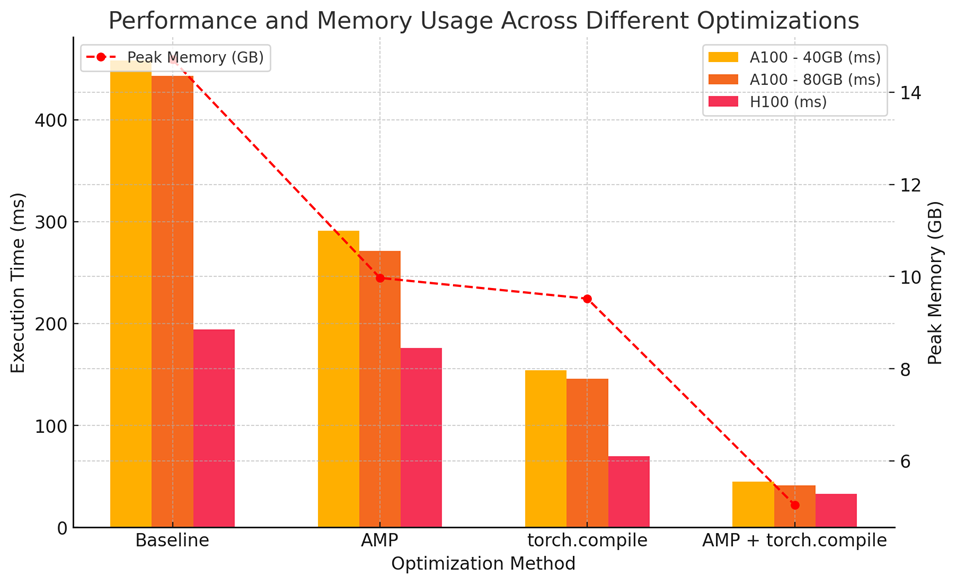
\includegraphics[width=0.8\linewidth]{figures/compute-opt.png}
    \caption{Computational efficiency of the \ignn~in terms of the execution time (left vertical axis) and peak memory (right vertical axis), measured using the baseline configuration, and configuration optimized with automated mixed precision (AMP), Just-In-time computation (JIT), and a combination of the two techniques. All measurements use graphs constructed with the Module Map MinMax method.}
    \label{fig:gnn-opt}
\end{figure}

The baseline configuration shows a latency of $\approx600$ ms/event on the A100 platform, and 264 ms/event on the H100 platform.
The H100's better performance is due to enhanced floating-point operation efficiency on FP32, namely 67 TFLOPS compared to 19.5 TFLOPS on the A100.
Under reduced precision, the latency is reduced by approximately 1/3 compared to the baseline on the A100, reaching on average 391 ms/event (40GB) and 362 ms/event (80GB), but only by a small margin on the H100, reaching 239 ms/event.
With JIT compilation, the execution time is enhanced to $\approx 200$ ms/event on both A100 platforms, and 92 ms/event on the H100.
Under the combined effect of both techniques, the execution time is significantly reduced to $\le 60$ ms/event across all platform. 

Table \ref{tab:gnn-comp-improve} shows the improvement in inference speed with respect to eager computation at full precision of each optimization. 
The A100 and H100 platforms respectively benefit from up to an 11x and 6x boost in efficiency. 
Remarkably, while the next-generation H100 outperforms the older A100-80GB by a factor of 2.25 in speed, this gap is shrunk to 1.40 by these optimizations. 
The larger enhancement of the A100 is an important benefit, because it is less expensive and power hungry than the new--generation counterpart, and hence more suitable for budget-constrained scientific computing. 
Interestingly, the performance boost delivered by the combined technique exceeds the product of the two underlying factors. 

\begin{table}[h!]
    \centering
    \begin{tabular}{|l|c|c|c|} \hline
        Optimization & {A100-40GB} & {A100-80GB} & {H100-80GB} \\ \hline\hline
        AMP & 1.57 & \textbf{1.63} & 1.10 \\
        Compilation & 2.97 & \textbf{3.02} & 2.77 \\
        Combined & 9.69 & \textbf{10.58} & 5.92 \\ \hline
    \end{tabular}
    \caption{Latency improvement over eager computation at full precision of each optimization, measured using the baseline configuration, and configurations optimized with automated mixed precision (AMP), JIT compilation, and a combination of both techniques. All measurements use graphs constructed with the Module Map MeanRMS method.}
    \label{tab:gnn-comp-improve}
\end{table}

Similarly, the peak memory consumption is significantly improved with the combined optimization.
Shown in figure \ref{tab:gnn-comp-improve}, the peak consumption on the A100 decreases from 19.16GB in the baseline to 6.48GB in the combined configuration, a factor of almost 3 smaller. 
Thanks to the reduced memory footprint, it becomes possible to simultaneously fit several events on the GPU and enhance the inference throughput, a logical next step for future computational optimization.
This direction is being explore using a \textit{inference-as-a-service} approach, which optimizes the GPU utilization by batching multiple inference events and processing
at the same time~\cite{zhao2025trackreconstructionservicecollider}. 

\newpage
\begin{figure}[h!]
    \centering
    \begin{subfigure}[b]{0.62\textwidth}
    \centering
        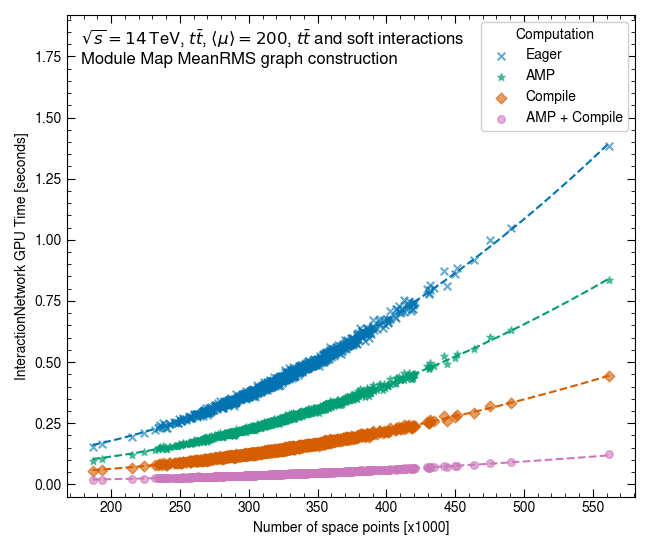
\includegraphics[width=\textwidth]{figures/rms_80g.png}
        \caption{}
        \label{subfig:gnn-time-node}
    \end{subfigure}

    \begin{subfigure}[b]{0.62\textwidth}\centering
        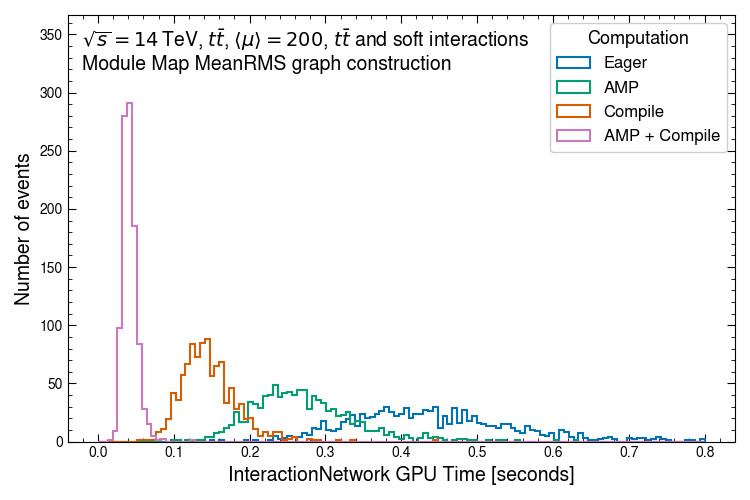
\includegraphics[width=\textwidth]{figures/rms_80g_hist.png}
        \caption{}
        \label{subfig:gnn-time-hist}
    \end{subfigure}
    \caption{GPU time of the \ignn~as a function of the number of space points in a $t\bar{t}$ event (a) and as a histogram (b), measured using the baseline configuration, and configurations optimized with automated mixed precision (AMP), JIT compilation, and a combination of both techniques. Each dashed line in (a) displays the best-fit second-order polynominal to the corresponding configuration. The fitted coefficients are exhibited in table \ref{tab:gnn-time-node-fit}. All measurements are performed on an NVIDIA-A100 GPU with 80 GB of memory, using graphs constructed with the Module Map MeanRMS method.}
    \label{fig:gnn-time-node}
\end{figure}


\begin{table}[ht]
    \centering
    \begin{tabular}{|l|c|c|c|} \hline
      {Computation}   &  {A} & {B} & {C} \\ \hline 
      \hline
       Eager  & 5.56 & $-8.73\times 10^{-1}$ & $1.30\times 10^{-1}$ \\
       AMP & 3.36 & $-5.40\times 10^{-1}$ & $8.87\times10^{-2}$ \\
       Compile & 1.73 & $-2.67\times 10^{-1}$  & $4.76\times 10^{-2}$ \\
       AMP + Compile & 0.457 & $-7.95\times 10^{-2}$ & $1.87\times 10^{-2}$ \\ \hline
    \end{tabular}
    \caption{The coefficients of a second-order polynomial fit to the GPU time shown in figure \ref{fig:gnn-time-node} for each optimization technique. The GPU time $t$ in units of seconds is assumed to depend on $x=\frac{\abs{V}}{10^6}$, where $V$ is the set of nodes, as $t=Ax^2+Bx+C$.}
    \label{tab:gnn-time-node-fit}
\end{table}
% \newpage
The event-level GPU run time as a function of the event size measured in the number of space points (graph nodes) along its best-fit second-order polynomial is shown in figure \ref{subfig:gnn-time-node}, and the fitted coefficients in table \ref{tab:gnn-time-node-fit}.
The majority of events contain 250,000 to 425,000 nodes, and their GPU time exhibits a well-defined scaling behaviour with respect to the number of space points in the event.
The dependence on space point number of GPU time scales quadratically, with a small linear component. 
Events far from the distribution core are well-described by the fitted curve, and no significant outliers are observed. 
The scaling behaviour is significantly improved with each optimization technique. 
In comparison to that of eager execution, the execution time of the combined AMP and Compilation execution scales much slower with event size, which is approximately proportional to true pile-up. 
This is evident, given the second-order coefficient of obtained from the latter $A_{AMP+Compile}=0.457$, being an order of magnitude smaller than former's corresponding coefficient $A_{Eager}=5.56$.
The execution time of the optimized code is thus not only small but also stays small over the typical range of pile-up.

The latency reduction from these computational optimizations is also evident from both the mean and spread of the GPU time distribution observed in each scenario, demonstrated in figure \ref{subfig:gnn-time-hist}.
In the combined optimization, the distribution averages to $42\pm 9$ ms, with a range of 103 ms, while in the eager baseline, the distribution centers at $443\pm117$ ms, with a range of 1231 ms. 
The former only only peaks at a lower latency, it is also much narrower than the latter.
This weak scaling makes the computation less susceptible to large events outside the core distribution, as shown in figure \ref{subfig:gnn-time-node} above $\abs{V}=4.5\times 10^5$.

% The rise in inference times as the event gets larger is also driven by the quadratic term

% [Discuss trend, strong/weak quadratic component]

\section{Pipeline computational performance}
\label{sect:pipeline-comp-perf}
The average latency of each stage in the GNN4ITk algorithm is shown in table \ref{tab:pipeline-comp-perf}, along with the average total execution time. 
The edge classification stage is measured with combined AMP and JIT optimization in all three variants.
Among the stages, graph segmentation is the slowest, contributing nearly 60\% of the total run time, while graph construction and edge classification each account for 20\%.
The difference in latency can be attributed to the different hardware on which these stages take place.
Graph construction in the Module Map method is carried out on the GPU, by means of a custom CUDA kernel that highly parallelizes many steps of the algorithm.
Edge classification leverages a graph neural network whose building blocks (the feed-forward multi-layer perceptron) are natively suitable to run on the GPU, and further benefit from the optimizations detailed in section \ref{sect:opt-techniques}.
As a result, both stages are optimized for and performed on the GPU, and are thus massively accelerated.
In comparison, the Walkthrough algorithm used in graph segmentation, originally conceived as an \textit{ad hoc} routine, contains many loops and logical \textsc{If-Then} statements (see section \ref{sect:walk}), and is thus difficult to parallelize.  
Although much effort has been put into optimizing the current implementation, a mechanism redesign that prioritizes parallelizability is necessary to accelerate it on the GPU and bring the entire GNN4ITk algorithm onto a single hardware architecture.
As of writing, a CUDA-based version of the Walkthrough is under development, promising better latency in the future. 
% its implementation are not GPU-friendly 

\begin{table}[h!]
    \centering
    \begin{tabular}{|l|c|c|c|} \hline
        \multirow{2}*{ Stage } & \multicolumn{3}{c|}{ Latency [ms/event] } \\ \cline{2-4}
         & MeanRMS& MinMax & Metric Learning\\ \hline\hline
        Graph construction & $41\pm 10$ & $41\pm 11$ & $932\pm 92$ \\
        Edge classification & $42\pm 9$ & $53\pm 12$ &  $47\pm10$  \\
        Graph segmentation & $120\pm 93$ & $120\pm 93$ &  \\ \hline \hline
        Total & $203\pm 94$ & &\\ \hline
    \end{tabular}
    \caption{Per-event run time of each stage in the GNN4ITk algorithm. The latency of graph construction and edge classification is evaluated on an NVIDIA-A100 GPU with 80GB of memory, and of graph segmentation on the AMD EPYC 7763 CPU, using graphs constructed with the Module Map MeanRMS method.}
    \label{tab:pipeline-comp-perf}
\end{table}
Of the two graph construction approaches, Module Map is significantly faster than Metric Learning.
The former is carried out by a custom CUDA-kernel which maximally parallelizes all steps of the graph creation on the GPU, most notably the \textsc{Merge/Join} operations of data frames,
which consume considerable computation on the CPU but are greatly accelerated on the GPU~\cite{cudf}.
On the other hand, the latter's graph construction latency is the sum of the metric learning and filter steps, both of which, as of writing, have not been optimized.
The metric learning step suffers from a lengthy kNN search in high a 12-dimensional space, and the filter step operates on large graphs of $\abs{V}\sim 6\times 10^6$ edges. 
These shortcomings are however optimizable, and methods to address them are being investigated. 
In the edge classification step, both graph construction approaches demonstrate similar speed, ranging from 42 to 53 ms/event.
Their difference in latency is evident from the average graph size, with $\abs{E}_{\mathrm{MinMax}} > \abs{E}_{\mathrm{ML}} > \abs{E}_{\mathrm{MeanRMS}}$, and correspondingly $t_{\mathrm{MinMax}} > t_{\mathrm{ML}} > t_{\mathrm{MeanRMS}}$, where $E$ is the edge set and $t$ the latency.
In the graph segmentation step, after fake edges are removed by a loose GNN score cut, the remaining graphs have similar edge set among the three variants, and their track building time is largely in accordance.

% Unlike the case of the tracking performance, it is not straightforward to compare the CKF- and GNN-based track finders in terms of the computing performance.
A comparison between the GNN- and the CKF-based track finders in terms of computing performance is unfortunately not straightforward.
The two algorithms by design operates on different hardware, the CKF on CPUs and the GNN on GPUs. 
The lack of a common benchmark is the main challenge, which stems from differences in architecture, programming models, and performance goals. 
For example, CPUs are optimized for low-latency execution of sequential tasks with a control flow, whereas GPUs for high-throughput executions of parallelized code.
These factors complicates the establishment of a fair and standardized metrics across the computing platforms. 
CPU performance is usually measured by the latency per task, and GPU performance by FLoating-point Operations Per Second (FLOPS).
% Even on CPUs, the HEP-SPEC06 benchmark used by the High-Energy Physics computing community \cite{Hepspec06} is based on but not identical to the industry standard and has no GPU equivalent.
Of course, one could naively compare the per-event latency of the two algorithms, and immediately runs into the question: \textit{\textbf{which}} latency? 
As we have seen in the previous section, the GNN latency varies widely with different GPU platforms, and the most performant platform may not be the choice for production infrastructure, giving little significance to this comparison. 
Quoting the latency of the CKF on different CPUs suffers from the same problem. 

Ultimately, the latency alone is insufficient to make a decision on the tracking technology in HL-HLC. 
It is not enough to answer the question \textit{``How fast can we reconstruct tracks?"}, but \textbf{How much does it cost to reach a certain event/second throughput using each algorithm?}
Therefore, a cost analysis taking into account all factors such as procurement, inherent throughput, latency, energy consumption, etc. is needed.
It necessitates investigations much deeper than the scope of the scope of this thesis.
For the moment, we refrain from making a direct comparison in computing performance between the two track finders.

\section{Toward computational performance in production environment}

The result in section \ref{sect:pipeline-comp-perf} representing the current computational performance of the GNN4ITk algorithm, is obtained from inference in a development environment.
Most of the source code is implemented in \textsc{Python}, and deep-learning models are written with \textsc{PyTorch}.
The Module Map, though implemented in C++ and CUDA, is incorporated via a python-binding into the inference pipeline.
The Walkthrough mechanism, though highly optimized by Just-In-Time compiling many components in a manner similar to C++ using \textsc{Numba}\cite{Numba}, is still implemented in \textsc{Python} code.
As a syntactically simple language rich in well-supported libraries, \textsc{Python} is suitable for research and development, but it is not the language of choice for production systems, which prioritize computational performance.
In fact, the legacy analysis software and the future tracking toolkit employed by ATLAS are both written in C++.
Therefore, table \ref{tab:pipeline-comp-perf} serves as the algorithm's baseline latency, not measurements in a realistic production environment.
As compiled C++ code is typically faster than the corresponding \textsc{Python} code, we expect even better performance than so far demonstrated. 

% To measure the execution time in production, further developments are needed.
% An inference pipeline must be implemented in \textsc{Athena}\cite{atlas_collaboration_2021_4772550}, which co

Further developments are needed to achieve competitive computing performance. 
The entire pipeline must be implemented in C++ and ported to \textsc{Athena}\cite{atlas_collaboration_2021_4772550}, enabling measurements and optimizations in production environment. 
All three stages of the Module Map variant have been integrated into the ACTS framework \cite{andreas_salzburger_2025_15260074}, which will become the tracking component of the ATLAS software. 
The graph construction stage of the Metric Learning remains to be accelerated and integrated. 
The slowest component of this step is the k-nearest-neighbor search which takes $\approx 400$ ms/event, due to the rather large 12-dimensional embedding space.
A possible method is to reduce the embedding dimensions by encouraging one for more dimensions to take a constant value using an extra loss term in training. 
During inference, the kNN search can ignore these dimension in the distance calculation, and therefore save time. 
The large number of edges, likely due to the current method being sub-optimal, is also a huge bottleneck, requiring a filter step to eliminate easy fake edges.
As Metric Learning is a mature technique of machine learning, more sophisticated models can better discriminate target hits from background, allowing to build smaller graphs and possibly bypass the Filter step. 


% \section{Discussion}
% 1. This is by no means a comprehensive account of all optimizations done to the GNN4ITk pipeline. In fact every stage of the algorithm has seen significant speed-up since its first appearance. This is the first time a configuration achieves 

% Ongoing work:
% \begin{itemize}
%     \item Inference pipeline integration into ATLAS and ACTS
%     \item Model compression
%     \item Fast Walkthrough
%     \item Throughput optimization 
% \end{itemize}
